\documentclass[a4paper,oneside,openany]{scrbook}

\usepackage[utf8]{inputenc}
\usepackage[T1]{fontenc}
\usepackage{graphicx}
\usepackage{amsmath}
\usepackage{amssymb}
\usepackage{booktabs}
\usepackage{url}
\usepackage{relsize}
\usepackage{hyperref}
\usepackage{libertine}
\usepackage[scaled=0.85]{beramono}
\usepackage{ifthen}
\usepackage{fancyhdr}
\usepackage{microtype}
\usepackage{xcolor}
\usepackage{float}
\usepackage{listings}
\usepackage[htt]{hyphenat}
\usepackage{tikz}
\usetikzlibrary{positioning,arrows.meta,calc,cipher,sponge}
\usepackage{subcaption}

\graphicspath{{../figures/}{./}}

\setlength{\emergencystretch}{3em}

\lstdefinestyle{codestyle}{
  basicstyle=\ttfamily\small,
  breaklines=true,
  breakatwhitespace=true,
  showstringspaces=false,
  frame=single,
  rulecolor=\color{black!25},
  backgroundcolor=\color{black!4},
  captionpos=b,
  numbers=none,
}
\lstset{style=codestyle}

% pandoc-generated chapters use \tightlist inside list environments
\providecommand{\tightlist}{\setlength{\itemsep}{0pt}\setlength{\parskip}{0pt}}

%%%%%%%%%%%%%%%%%%%%%%%%%%%%%%%%%%%%%%%%%%%%%%%%%%%%%%%%%%%%%%%%%%%%%%%%%%%%%%%%
% Replace these values
%%%%%%%%%%%%%%%%%%%%%%%%%%%%%%%%%%%%%%%%%%%%%%%%%%%%%%%%%%%%%%%%%%%%%%%%%%%%%%%%
\newcommand{\thesistitleDE}{Leichtgewichtige Kryptographie auf ressourcenbeschränkten ARM-Mikrocontrollern:\\Benchmark-Vergleich von Ascon-AEAD128 und AES-128-GCM}
\newcommand{\thesistitleEN}{Lightweight Cryptography on Constrained ARM Microcontrollers:\\A Benchmark Comparison of Ascon-AEAD128 and AES-128-GCM}
\newcommand{\student}{Johannes Zipper}
\newcommand{\matrnr}{22411902}
\newcommand{\stammnr}{} % Unset this variable if you only have a (single) matriculation number
\newcommand{\submissiondate}{29.\ July 2026}
\newcommand{\supervisor}{Prof.~Dr.~Martin Schramm}
\newcommand{\secsupervisor}{Tobias Spieker} % Unset this variable if no second supervisor is required
\newcommand{\faculty}{Angewandte Informatik}

% Select your course of studies here
\newcommand{\studies}{Bachelor Cybersecurity}
%\newcommand{\studies}{Bachelor Künstliche Intelligenz}
%\newcommand{\studies}{Bachelor Angewandte Informatik}
%\newcommand{\studies}{Master Angewandte Informatik}
%\newcommand{\studies}{Bachelor Elektro- und Informationstechnik}
%\newcommand{\studies}{Master Elektro- und Informationstechnik}
%\newcommand{\studies}{Bachelor Medientechnik}
%\newcommand{\studies}{Master Medientechnik}
%\newcommand{\studies}{Master of Applied Research}

% Select the targeted degree here
%\newcommand{\degree}{Bachelor of Engineering (B.Eng.)}
%\newcommand{\degree}{Master of Engineering (M.Eng.)}
%\newcommand{\degree}{Master of Science (M.Sc.)}
\newcommand{\degree}{Bachelor of Science (B.Sc.)}
%%%%%%%%%%%%%%%%%%%%%%%%%%%%%%%%%%%%%%%%%%%%%%%%%%%%%%%%%%%%%%%%%%%%%%%%%%%%%%%%

\renewcommand*{\UrlFont}{\ttfamily\smaller\relax}

\begin{document}
\pagestyle{headings}
\pagenumbering{roman}
\input{title}

\chapter*{Abstract}
\addcontentsline{toc}{chapter}{Abstract}
Authenticated encryption is a baseline requirement for in-vehicle
communication. Standards such as AUTOSAR SecOC define message authentication
across the vehicle network, and ISO/SAE 21434 places such measures inside a
documented cybersecurity risk management process. In practice the algorithm
used is almost always AES in Galois/Counter Mode. A large share of automotive
nodes, however, are low-cost 32-bit microcontrollers without a hardware
cryptographic accelerator. On these parts AES-128-GCM runs entirely in
software, including the GHASH field multiplication, which maps poorly onto a
minimal instruction set. NIST standardized Ascon in SP 800-232 as a lightweight
alternative, but quantitative performance data on representative Cortex-M
hardware is scarce. This work addresses that gap.

The evaluation uses the NUCLEO-F072RB (Cortex-M0, 128 KB Flash, 16 KB SRAM)
and the NUCLEO-L476RG (Cortex-M4F), with the Cortex-M4F clocked at 48 MHz to
match the Cortex-M0 ceiling, so that timing differences reflect architecture
rather than clock frequency. Both algorithms are measured as software-only
implementations, using the official Ascon reference code and mbedTLS 3.6.2.
mbedTLS is configured with the small four-bit GHASH table, which is the
memory-frugal configuration of AES-GCM rather than its speed ceiling. Execution
time is taken from a 32-bit free-running timer at one tick per cycle, with
interrupts masked and one warmup iteration discarded. Both implementations are
verified against published known-answer test vectors on target. The matrix
covers message sizes from 1 to 10\,000 bytes and the optimization levels -O0
through -Os.

Ascon-AEAD128 was faster than AES-128-GCM at every measured message size, on
both boards, and at every optimization level. The advantage appears in the
fixed per-call cost that dominates short messages and in the per-byte cost that
dominates long messages, so it does not depend on the message profile of the
application. The largest ratio is approximately 4.6 in favor of Ascon-AEAD128,
at -O1 and -O2 on the Cortex-M0, against approximately 2.0 on the Cortex-M4F.

At -Os, the level a memory-constrained deployment would realistically choose,
AES-128-GCM required approximately 3.8 times the Flash of Ascon-AEAD128 on both
boards. At -O1 through -O3 the relation inverts, because the compiler unrolls
the permutation, so the speed advantage and the code-size advantage are
obtained together only when building for size. Within the reported build
configuration the results give a quantitative basis for preferring
Ascon-AEAD128 on constrained, software-only targets, with the advantage growing
as the target becomes more constrained.

\chapter*{Declaration on the Use of AI-Based Tools}
\addcontentsline{toc}{chapter}{Declaration on the Use of AI-Based Tools}

AI-based tools were used in the preparation of this thesis. The nature and
extent of that use is listed below:

\begin{itemize}
  \item \textbf{Claude (Anthropic), models Claude Opus 4.5 and Claude Opus 5:}
        drafting and linguistic revision of text based on my own outlines and
        my own measurement data, condensing of existing sections, suggestions
        for chapter structure, support with LaTeX formatting and figure
        integration, and debugging of the analysis scripts.
\end{itemize}

The conception of the work, the design of the measurement setup, the execution
of all measurements, and the evaluation and interpretation of the results are
my own. All text produced or revised with AI-based tools was reviewed by me for
accuracy, corrected where necessary, and is my responsibility. No measurement
values, results, or bibliographic references were generated by AI tools.

\vspace{2cm}
\noindent\rule{6cm}{0.4pt}\\
Deggendorf, \today \qquad Johannes Zipper


\tableofcontents
\listoffigures
\listoftables

\cleardoublepage%
\setcounter{page}{1}
\pagenumbering{arabic}
\chapter{Introduction}

\section{Cryptography in the Automotive Domain}

Modern vehicles are no longer purely mechanical systems.
Today's cars contain upwards of hundreds of Electronic Control Units (ECUs)
responsible for functions ranging from engine management and brake control to
infotainment, over-the-air software updates, and vehicle-to-everything
communication.
Due to the sheer number of features, these systems are increasingly
interconnected.
All connections can be separated into two categories: internal ones, which are
mostly bus protocols such as CAN, LIN, and Automotive Ethernet, and external
ones such as V2X and telematics interfaces.
These circumstances increase the attack surface exposed to adversaries.
A successful intrusion into a safety-relevant ECU carries consequences that
extend well beyond data loss: it can compromise brake controllers, manipulate
steering actuators, or falsify sensor data, directly endangering human lives.

Cryptographic protection of ECU communication is therefore not optional.
Standards such as AUTOSAR SecOC (Secure Onboard Communication) and
ISO/SAE~21434 establish requirements for message authentication and
confidentiality across the vehicle network.
In practice, the algorithm most commonly used to fulfill these requirements is
the Advanced Encryption Standard (AES).
It has served as the global symmetric encryption standard since its NIST
standardization in 2001~\cite{FIPS197} and is deeply embedded in automotive
security stacks, ranging from hardware security modules (HSMs) to communication
middleware.

\section{Cryptographic Requirements of Modern ECUs}

ECUs span a wide spectrum of computational capability.
On the high end are domain controllers managing ADAS functions or running an
automotive-grade operating system; these may be equipped with multi-core
processors, dedicated cryptographic co-processors, and several megabytes of RAM.
At the other end are simple body control modules, sensor nodes, and actuator
controllers built around low-cost 32-bit microcontrollers with RAM measured in
tens of kilobytes and no hardware cryptographic accelerator.
On these devices the computational cost of cryptographic operations becomes a
real concern.

For such constrained ECUs, the cryptographic primitive must satisfy several
requirements simultaneously: it must provide authenticated encryption with
associated data (AEAD) to guarantee confidentiality, integrity, and authenticity
in a single pass; it must execute within a time budget that does not interfere
with real-time control tasks; and its implementation must fit within the
available Flash and RAM without displacing application code.
These requirements motivate a closer examination of whether AES-128-GCM ---
designed for general-purpose hardware --- remains the most appropriate choice
for every node in the vehicle network, or whether purpose-built lightweight
alternatives deserve consideration.

\section{The Limits of AES on Low-End Microcontrollers}

AES-128-GCM is the dominant AEAD construction in modern security protocols and
is well understood with respect to both security and implementation.
On hardware that includes a dedicated AES accelerator, it executes efficiently
and introduces negligible overhead.
However, a large portion of automotive microcontrollers --- particularly those
in cost-sensitive, high-volume applications --- are based on simple 32-bit cores
such as the ARM Cortex-M0, which provide no hardware cryptographic acceleration.
On these platforms, a software implementation of AES-128-GCM must perform the
full AES key schedule and block cipher in software, and the GCM authentication
step requires a 128-bit polynomial multiplication (GHASH) that maps poorly onto
a minimal instruction set without hardware multiply-accumulate support.
The result can be an implementation that is slower, larger in code size, or more
energy-intensive than the available budget permits.

This raises a practical engineering question: for constrained ECUs where AES
hardware acceleration is absent, is there a standardized alternative that offers
better performance characteristics without sacrificing security?

\section{The NIST Lightweight Cryptography Standardization Process}

Recognizing the growing need for cryptographic primitives suited to constrained
devices, NIST initiated a Lightweight Cryptography (LWC) standardization project
in 2018~\cite{NISTLWCCall}.
In February 2023, NIST announced \mbox{ASCON} as the winner~\cite{ASCON2023}.
ASCON is a family of lightweight cryptographic algorithms based on a sponge
construction, designed from the ground up for efficient software implementation
on small processors.
Its selection provides the embedded and automotive security community with a
standardized, well-analyzed alternative to AES-GCM for use cases where resource
constraints are the primary concern.

Despite this standardization, ASCON adoption in automotive and industrial
embedded systems remains limited.
AES continues to dominate deployed security stacks, in part due to inertia,
existing hardware support, and a lack of quantitative performance data on
representative automotive-class microcontrollers.
This work aims to contribute directly to closing that gap.

\section{Objective and Research Questions}

This paper presents a quantitative benchmark comparing Ascon-AEAD128 and
AES-128-GCM on two ARM Cortex-M microcontrollers representative of the
low-to-mid range of the automotive ECU spectrum: the NUCLEO-F072RB
(Cortex-M0, 48\,MHz) and the NUCLEO-L476RG (Cortex-M4F, 80\,MHz).
Both boards serve as a simulation of the resource conditions found in
constrained automotive ECUs.
All measurements use software-only implementations to ensure a fair,
hardware-accelerator-independent comparison applicable to the broadest range of
real-world deployments.

The following research questions guide the study:
\begin{enumerate}\tightlist
  \item \textbf{Performance:} How do Ascon-AEAD128 and AES-128-GCM compare in
        execution time and throughput across a range of message sizes on each
        platform?
  \item \textbf{Flash footprint:} What is the Flash code-size footprint of each
        implementation relative to the constraints of a typical automotive
        microcontroller?
  \item \textbf{Optimization sensitivity:} How does compiler optimization level
        affect the relative performance of the two algorithms?
  \item \textbf{Architecture dependence:} Does the performance gap between the
        two algorithms differ between the Cortex-M0 and the Cortex-M4F, and what
        does this imply for ECU selection?
\end{enumerate}

\section{Structure of This Paper}

The remainder of this paper is organized as follows.
Chapter~2 provides the technical background on AES-128-GCM, the ASCON family,
and the target hardware platforms.
Chapter~3 describes the benchmark methodology, including the measurement setup,
timing approach, library selection, and build configuration.
Chapter~4 presents the measurement results.
Chapter~5 discusses the findings in the context of the research questions and
draws practical conclusions for algorithm selection on constrained automotive
hardware.
Chapter~6 concludes the paper and outlines directions for future work.

\chapter{Background}

\section{Authenticated Encryption with Associated Data (AEAD)}

Cryptographic protocols for embedded communication commonly require three
security objectives simultaneously: confidentiality (to prevent unauthorized
reading of the message), integrity (to detect any modification during
transmission), and authenticity (to verify that the message originates from a
legitimate sender).
Traditionally, these properties were achieved by combining a separate cipher
with a message authentication code (MAC).
However, the secure composition of two independent primitives is non-trivial:
the order of operations matters, and incorrect combinations can introduce
vulnerabilities even when each primitive is individually sound.
Authenticated Encryption with Associated Data (AEAD) addresses this by combining
all three objectives into a single, unified primitive.

An AEAD scheme takes four inputs: a secret key~$K$, a nonce~$N$ (a value that
must be unique per encryption under a given key), a plaintext message~$M$, and a
block of associated data~$AD$.
The associated data is authenticated but not encrypted: it remains readable in
the clear while being bound to the ciphertext via the authentication tag.
The scheme produces a ciphertext~$C$ and an authentication tag~$T$.
Decryption takes the same key and nonce, as well as the ciphertext, tag, and
associated data, and returns the recovered plaintext only if the tag verifies
successfully; otherwise it returns an explicit failure.
This fail-closed behavior is essential in embedded contexts, since a receiver
that processes unauthenticated data before verification completes is vulnerable
to plaintext-dependent side channels and fault injection.

For the constrained microcontroller setting considered in this work, two AEAD
properties are of particular practical relevance.
First, single-pass processing absorbs plaintext and produces the authentication
tag in one sequential pass over the data, minimizing RAM requirements by
avoiding the need to buffer the full message.
Second, a compact state and key schedule reduce code size and initialization
overhead, both of which are essential on devices with limited Flash.
These properties will later serve as evaluation criteria when comparing
AES-128-GCM and Ascon-AEAD128.

\section{AES-128-GCM}

\subsection{The AES Block Cipher}

The Advanced Encryption Standard (AES) is a substitution-permutation block
cipher standardized by NIST in 2001~\cite{FIPS197}.
It operates on a fixed block size of 128 bits and supports key lengths of 128,
192, or 256 bits; this work uses the 128-bit key variant exclusively
(AES-128).
The cipher applies ten rounds of transformation to a $4\times4$ byte state
matrix.
Each round consists of four operations: \texttt{SubBytes} (a non-linear byte
substitution via the AES S-box), \texttt{ShiftRows} (a cyclic shift of state
rows), \texttt{MixColumns} (a linear diffusion step operating on state columns
in $\mathrm{GF}(2^8)$), and \texttt{AddRoundKey} (XOR of the state with a
round-specific subkey).
The 128-bit key is expanded into eleven round keys before encryption begins,
a process known as the key schedule.

The security of AES rests on more than two decades of public cryptanalysis; no
practical attack against the full cipher is known.
With hardware acceleration (a dedicated AES engine), the cipher executes at
throughputs measured in gigabits per second.
On a software-only Cortex-M0 implementation, however, the \texttt{MixColumns}
step and the S-box lookups impose a considerable cycle cost, because the M0
lacks the wider data path and lookup acceleration found on higher-end cores.
This performance gap on minimal instruction-set architectures is the central
motivation for evaluating a lightweight alternative.

\subsection{Galois/Counter Mode (GCM)}

AES alone is a block cipher and not an AEAD scheme: it encrypts exactly one
128-bit block and provides no authentication.
Galois/Counter Mode (GCM) combines AES in counter mode (CTR) for encryption
with a polynomial hash (GHASH) for authentication, yielding an AEAD
construction~\cite{NISTSP80038D}.

In CTR mode, a counter value is encrypted by AES and the resulting keystream
block is XORed with the plaintext.
The counter is incremented for each successive block, which enables
parallelized encryption independent of plaintext content.
GHASH computes a 128-bit authentication tag using polynomial operations over
the ciphertext blocks and associated data in $\mathrm{GF}(2^{128})$, a finite
field defined over 128-bit values.
The hash key~$H$ is derived by encrypting a zero block under the session key
at initialization.

GCM's parallelizability is its primary advantage on general-purpose hardware
with wide data paths.
Its principal weakness on constrained processors is the GHASH step:
multiplication in $\mathrm{GF}(2^{128})$ requires either a hardware carry-less
multiply instruction or a software implementation using multiple 32-bit
operations.
The Cortex-M0 provides only a 32-bit multiply without a carry-less variant, so
a software GHASH implementation on that core requires a series of XOR and shift
operations that contribute noticeably to the total cycle count.
Additionally, GCM requires a unique nonce per encryption; nonce reuse under the
same key is catastrophic, recovering both the hash key and the plaintext with a
small number of observed ciphertexts.

\subsection{Software-Only Scope}

The STM32L476RG does not include a hardware AES peripheral; that block is
present only in the STM32L486 and related parts of the same product family, as
confirmed by the device reference manual.
Both benchmark boards therefore present an identical software-only execution
environment for this comparison.
The absence of a hardware cryptographic accelerator on the selected boards is a
deliberate design choice: restricting the comparison to software implementations
throughout makes the results applicable to the broad class of constrained 32-bit
microcontrollers that ship without vendor-specific AES acceleration, which
represents the majority of cost-sensitive automotive nodes.

\section{The ASCON Family}

\subsection{The ASCON Permutation}

All ASCON variants use the same underlying permutation, written as $p^a$ or
$p^b$ depending on how many rounds are applied.
The permutation operates on a 320-bit state organized as five 64-bit words
$x_0$ through $x_4$.
Each round applies three layers in sequence.

The first layer, $p_C$ (constant addition), XORs a round-specific constant into
word~$x_2$, introducing asymmetry between rounds to prevent slide attacks.
The second layer, $p_S$ (substitution), applies a 5-bit S-box in parallel to
all 64 bit-sliced positions across the five state words.
This S-box provides non-linearity with simple arithmetic and was chosen for the
efficiency of its bitsliced implementation on processors with native 64-bit or
32-bit word operations.
The third layer, $p_L$ (linear diffusion), applies independent linear
transformations to each of the five state words using rotations and XOR,
ensuring that differences propagate rapidly across the full state.

The full ASCON permutation uses twelve rounds ($p^{12}$) for initialization and
finalization.
The internal data-processing step uses eight rounds ($p^8$) for Ascon-AEAD128.
On 32-bit microcontrollers the five 64-bit state words are held in pairs of
32-bit registers, so the rotation-and-XOR structure of the linear layer maps
efficiently onto the available register file without memory traffic.

\subsection{Sponge and Duplex Construction}

ASCON uses a sponge-based construction --- specifically the duplex variant ---
rather than the block-cipher-mode approach used by AES-GCM.
The sponge model divides the state into two parts: the rate~$r$ (the part that
interfaces with input and output) and the capacity~$c$ (the part that remains
hidden from I/O, forming the security margin).
For Ascon-AEAD128, the rate is 128 bits and the capacity is 192 bits, giving a
total state of 320 bits.

In the duplex variant used for AEAD, plaintext is XORed into the rate portion of
the state one rate-sized block at a time, followed by the permutation.
The ciphertext is extracted from the state after the absorption, mixing
encryption and authentication in a single sequential pass.
This single-pass property means that memory buffering of the full message is
never required, a significant advantage over constructions that must process the
ciphertext twice (once for decryption, once for authentication).

The capacity portion of the state is never directly observable by an attacker
and provides the security guarantee.
For Ascon-AEAD128, the 192-bit capacity yields a claimed security level of
128 bits against generic attacks on both confidentiality and integrity.

\subsection{Ascon-AEAD128}

Ascon-AEAD128 is the primary AEAD member of the ASCON family and the algorithm
selected as the NIST Lightweight Cryptography standard~\cite{ASCON2023}.
It accepts a 128-bit key, a 128-bit nonce, associated data of arbitrary length,
and a plaintext of arbitrary length, and produces a ciphertext of the same
length as the plaintext together with a 128-bit authentication tag.

The processing pipeline proceeds in four phases.
In the initialization phase, the 320-bit state is assembled from the key, nonce,
and algorithm-specific initialization vector, then transformed by $p^{12}$.
In the associated data phase, the associated data is absorbed into the rate in
128-bit blocks, each followed by $p^8$; the last block is padded, and a domain
separation constant is XORed into the state at the end of this phase.
In the encryption phase, plaintext blocks are absorbed and ciphertext blocks are
extracted in the same pass, each followed by $p^8$.
In the finalization phase, the key is XORed into the state, $p^{12}$ is applied,
and the authentication tag is extracted from the last 128 bits of the state.

For the benchmark in this work, Ascon-AEAD128 is evaluated using the official
ASCON reference implementation in C~\cite{ASCONSoftware}.

\subsection{Ascon-Hash256}

Ascon-Hash256 is the hash function member of the ASCON family.
It produces a 256-bit digest from an input of variable length using the same
$p^{12}$ permutation as Ascon-AEAD128.
Message absorption proceeds in 64-bit rate blocks, each followed by $p^{12}$,
and the digest is squeezed in two 64-bit output blocks after all input has been
absorbed.


\subsection{Ascon-80pq and the Post-Quantum Outlook}

Ascon-80pq is a variant of Ascon-AEAD128 that extends the key length from
128 to 160 bits while keeping the nonce at 128 bits and the tag at 128 bits.
The longer key is a precautionary measure against Grover's algorithm, which
effectively halves the security level of a symmetric key in bits against an
adversary with a large-scale quantum computer.
A 128-bit key offers approximately 64-bit post-quantum security under Grover's
model, while the 160-bit key of Ascon-80pq provides approximately 80-bit
post-quantum security.

The performance overhead of the 160-bit key variant relative to Ascon-AEAD128
is limited to initialization, where the additional 32 bits are incorporated into
the state setup.
The permutation rounds and data processing phases are identical.
Ascon-80pq is therefore of interest as a forward-compatible migration path for
automotive security architectures that must account for long vehicle service
lifetimes, during which the practical capabilities of quantum computing may
evolve.
Ascon-80pq is part of the original ASCON v1.2 competition submission and is not
included in NIST SP~800-232, which standardizes only Ascon-AEAD128,
Ascon-Hash256, Ascon-XOF128, and Ascon-CXOF128~\cite{ASCONSpec}.

\section{Architectural Comparison: Sponge vs.\ Block Cipher + GCM}

The structural differences between AES-128-GCM and Ascon-AEAD128 have concrete
implications for software performance on constrained microcontrollers, which are
worth making explicit before the benchmark results are presented.

AES-128-GCM is built from two largely independent components: the AES block
cipher and the GHASH authenticator.
Each has its own state, key material, and processing requirements.
The AES key schedule expands 128 bits into 176 bytes of round keys that must
either be precomputed and stored in RAM or recomputed for each execution.
The GHASH state requires an additional 128-bit accumulator and the hash key~$H$.
On a Cortex-M0 without hardware multiply, GHASH is the performance bottleneck
for short messages, since its initialization cost (one AES block encryption) is
spread poorly at small input sizes.

Ascon-AEAD128 holds its entire state in the 320-bit permutation input.
There is no separate key schedule: the key is absorbed directly into the state
during initialization.
The permutation is defined entirely by bitwise rotations and XOR, operations
that are cheap on any 32-bit or 64-bit processor without specialized hardware.
The absence of S-box table lookups also eliminates a class of cache-timing
side channels that must be considered when deploying AES on processors without
constant-time hardware support.

Both algorithms process data in 128-bit units per core operation: AES encrypts
one 128-bit block per cipher call, and Ascon-AEAD128 absorbs one 128-bit rate
block per permutation call.
The throughput difference between them therefore cannot be attributed to a rate
disadvantage on either side and must be found in the per-operation cost of the
underlying primitive.
Whether Ascon-AEAD128 or AES-128-GCM requires fewer cycles on a given platform
cannot be determined theoretically; answering it quantitatively is the central
goal of this benchmark.

\section{Target Platforms}

\subsection{ARM Cortex-M0 --- NUCLEO-F072RB}

The NUCLEO-F072RB board is built around the STM32F072RB microcontroller, which
integrates an ARM Cortex-M0 core clocked at 48\,MHz.
The Cortex-M0 is the smallest and most constrained member of the ARM Cortex-M
family.
It implements the ARMv6-M instruction set architecture, a minimal 16/32-bit
Thumb instruction set without the DSP extensions, floating-point unit, or
hardware divide instruction present in larger M-class cores.
The core has no instruction or data caches.

Relevant characteristics for this benchmark include the absence of a hardware
multiply-accumulate that would accelerate GHASH, a two-cycle latency for the
available $32\times32$-bit multiply (which produces a 32-bit result), and the
lack of a Data Watchpoint and Trace (DWT) unit with a cycle counter.
Because the DWT cycle counter is not present on the M0, cycle-accurate
measurement on this board uses TIM2, configured as a 32-bit free-running counter
driven by the system clock.

The F072RB is representative of the lowest tier of 32-bit microcontrollers
found in automotive body and sensor applications, where unit cost and power
consumption are the dominant design constraints.

\subsection{ARM Cortex-M4F --- NUCLEO-L476RG}

The NUCLEO-L476RG board is built around the STM32L476RG microcontroller, which
integrates an ARM Cortex-M4F core clocked at up to 80\,MHz.
The Cortex-M4F implements the ARMv7E-M instruction set architecture, which
extends ARMv6-M with DSP-oriented instructions including a single-cycle
$32\times32$-bit multiply with 64-bit accumulate (\texttt{MLA},
\texttt{SMLAL}), single-instruction saturating arithmetic, and a
single-precision floating-point unit (FPU).
The core also includes an Adaptive Real-Time (ART) memory accelerator, which
implements an instruction prefetch buffer and a branch cache to reduce Flash
access latency at high operating frequencies.

For timing, the Cortex-M4F provides a DWT unit including the
\texttt{DWT->CYCCNT} cycle counter, a 32-bit register incremented on every
processor clock, readable with a single memory-mapped register access.

The L476RG is representative of a mid-range automotive microcontroller, suitable
for body control modules and sensor fusion nodes with moderate processing
requirements.
Together with the F072RB, the two boards span a performance range relevant to
the lower half of the automotive ECU spectrum.

\section{Related Work}

Performance comparisons between ASCON and AES-GCM on embedded hardware have
appeared in several contexts since ASCON's selection as the NIST LWC standard.
Benchmarks conducted on AVR 8-bit and MSP430 16-bit platforms during the NIST
LWC competition evaluation process demonstrated ASCON's advantage on
ultra-constrained targets, but these results are not directly applicable to
32-bit ARM Cortex-M deployments that represent the current generation of
automotive microcontrollers.

Work targeting ARM Cortex-M platforms specifically has been published both by
the ASCON team and by independent researchers.
The ASCON team provides cycle counts for their reference and optimized
implementations on several Cortex-M targets~\cite{ASCONSoftware}.
However, published figures often report single-point measurements at a fixed
message length rather than throughput curves across a logarithmic range of input
sizes, which are needed to characterize behavior for the short messages typical
in automotive CAN frames and sensor update packets.

To the authors' knowledge, no published work directly compares AES-128-GCM and
Ascon-AEAD128 across both a Cortex-M0 and a Cortex-M4F target with a
controlled, software-only methodology that includes compiler optimization level
as an explicit variable.
This work aims to fill that gap by providing reproducible benchmark data for
both platforms under a unified measurement framework.

\chapter{Methodology}

\section{Overview and Experimental Design}

This chapter describes how the benchmark was constructed and how every reported
number was produced.
The goal is a fair and reproducible comparison of Ascon-AEAD128 and AES-128-GCM
under matched conditions on two constrained microcontrollers.
Fairness here has a precise meaning: both algorithms run as software-only
implementations, both are measured through an identical timing harness, both are
compiled with the same toolchain and the same set of optimization levels, and the
one-time setup cost is excluded from the timed region for both in the same way.

The experimental design varies four factors: the algorithm (Ascon-AEAD128 or
AES-128-GCM), the hardware platform (Cortex-M0 or Cortex-M4F), the input
message size (swept across several orders of magnitude), and the compiler
optimization level (swept from no optimization through size optimization).
Each combination is measured many times and reduced to summary statistics
offline.
Code size is measured separately, as a static property of the compiled binaries
rather than a runtime measurement.

\section{Target Platforms}

Two STMicroelectronics Nucleo-64 development boards represent the low and
middle of the constrained range.
Their relevant properties are summarized in Table~\ref{tbl:platforms}.
Both boards expose an on-board ST-LINK debugger with a USB virtual COM port
routed to USART2, which carries the measurement output.

\begin{table}[htbp]
  \centering
  \caption{Target platform properties}
  \label{tbl:platforms}
  \begin{tabular}{lll}
    \toprule
    Property              & NUCLEO-F072RB     & NUCLEO-L476RG    \\
    \midrule
    Microcontroller       & STM32F072RBT6     & STM32L476RGT6    \\
    Core                  & Cortex-M0         & Cortex-M4F       \\
    Maximum clock         & 48\,MHz           & 80\,MHz          \\
    Flash                 & 128\,KB           & 1\,MB            \\
    SRAM                  & 16\,KB            & 128\,KB          \\
    Hardware AES          & None              & None             \\
    Cycle counter (DWT)   & Absent            & Present          \\
    Instruction prefetch  & None              & ART accelerator  \\
    Floating-point unit   & None              & Single precision \\
    \bottomrule
  \end{tabular}
\end{table}

\subsection{NUCLEO-F072RB (Cortex-M0)}

The F072 carries a Cortex-M0 core with no hardware multiplier for wide
operands, no instruction cache, no branch predictor, and no floating-point
unit.
It represents the lower end of the device range, where every cycle and every
kilobyte is scarce.
Its 16\,KB of SRAM is the binding constraint on this study, and it limits the
largest message size that can be benchmarked on this board.

\subsection{NUCLEO-L476RG (Cortex-M4F)}

The L476 carries a Cortex-M4F core with a single-cycle hardware multiplier, a
single-precision floating-point unit, and the ST ART accelerator, which
prefetches and caches instructions from Flash.
It represents the middle of the range.
The L476 has substantially more memory than the F072, so memory is not a
constraint on this board, but it is included to expose how the relative
performance of the two algorithms depends on the processor architecture.

The specific part on the NUCLEO-L476RG does not contain a hardware AES block;
only the L486 and related parts in the same family include one.
This absence is useful for the study, because it means there is no hardware
cryptographic path that could be engaged accidentally, so the software
comparison is consistent on both boards.

\subsection{Clocking and the Matched-Frequency Decision}

Both boards run at 48\,MHz for the timing comparison.
The L476 is capable of 80\,MHz, so it is intentionally underclocked to the
F072 ceiling.
This choice removes clock frequency as a variable: any difference in measured
time between the two boards at the same clock then reflects the processor
architecture alone, not a difference in operating frequency.

The measurements are reported primarily as cycle counts rather than wall-clock
time, since the timer increments once per processor clock (see
Section~\ref{sec:timing-source}), so one timer tick equals one clock cycle and
the cycle count is independent of the operating frequency.

\section{Toolchain and Build System}

All firmware was built with a single toolchain to keep the comparison
consistent.
The compiler is \texttt{arm-none-eabi-gcc} version 14.3.1, supplied with the
STM32CubeCLT bundle.
The build is driven by CMake with the Ninja generator, both bundled with
CubeCLT.
Project skeletons, including peripheral initialization and the linker script,
were generated with STM32CubeMX configured for CMake output.
The host operating system was Windows.

The base compiler flags follow the CubeMX template.
They include \texttt{-ffunction-sections}, \texttt{-fdata-sections}, and linker
garbage collection (\texttt{-Wl,--gc-sections}), the size-oriented newlib-nano
C library (\texttt{--specs=nano.specs}), and the architecture flags appropriate
to each core.
On the L476 these include the hardware floating-point ABI, although
floating-point arithmetic is not used by either algorithm.

The optimization level is the one build variable that changes across the
measurement matrix.
It is controlled through a single CMake cache variable set per build preset.
Each preset reconfigures the build at one optimization level, from \texttt{-O0}
through \texttt{-Os}, so that the same source produces a family of binaries
that differ only in optimization.

\section{Cryptographic Implementations}

Both implementations are taken from existing open-source projects rather than
written for this study.
This keeps the comparison representative of what a developer would actually
deploy, and it avoids the risk of an unrepresentative hand-written
implementation favoring one side.

\subsection{AES-128-GCM (mbedTLS)}

AES-128-GCM is provided by mbedTLS version 3.6.x~\cite{mbedTLS}.
mbedTLS was selected because it is a widely deployed, well-maintained library
with a complete and verified AES-GCM implementation, which lends the comparison
credibility.
The library was reduced to a minimal configuration containing only the modules
required for AES-128-GCM.

Three configuration choices affect the measurements and are disclosed here,
because the reported numbers are only interpretable alongside them.

First, the small four-bit GHASH multiplication table is used.
The larger eight-bit table is faster per byte but enlarges the GCM context by
roughly 3.8\,KB of RAM.
The small table was chosen because it represents a genuinely lightweight
configuration of AES-GCM, matching the constrained-device framing of this work.
As a consequence, the reported AES-GCM throughput represents the memory-frugal
end of what mbedTLS can achieve rather than its speed ceiling.
This point is revisited in the discussion.

Second, the AES lookup tables are placed in Flash rather than generated in RAM
at initialization.
This shifts roughly 8\,KB from RAM to Flash, which is the realistic trade-off
on a part with only 16\,KB of SRAM.
It affects the code-size results but has no meaningful effect on runtime.

Third, only the 128-bit key length is compiled.
The 192-bit and 256-bit key schedules are removed.
Because only AES-128 is benchmarked, this has no effect on runtime and only a
small effect on Flash size.

\subsection{Ascon-AEAD128 (Reference Implementation)}

Ascon-AEAD128 is provided by the official ASCON reference implementation in
C~\cite{ASCONSoftware}.
The reference variant was chosen over the optimized variants for portability and
because it corresponds directly to the standardized specification.
The implementation uses a 16-byte key, a 16-byte nonce, and produces a 16-byte
authentication tag, with a rate of 16 bytes.

The choice of the reference variant has a visible effect on code size at high
optimization levels.
This is reported and discussed rather than hidden, because it reflects what a
developer integrating the standard reference code would observe.

\subsection{Uniform Wrapper Interface}

Each implementation is reached through a thin wrapper with a matching
signature, so that the benchmark harness calls both algorithms the same way.
The AES wrapper separates key setup from encryption, so that the one-time key
schedule can be hoisted out of the timed region.
The ASCON single-pass AEAD interface has no separable key schedule, so its
encryption call is timed in full.
Neither wrapper performs additional copying inside the timed path beyond what
the underlying library requires.

\section{Correctness Verification}

No timing measurement was trusted until the implementation producing it was
shown to be correct.
Each algorithm was checked against a published Known Answer Test vector, the
NIST GCM vector for AES-128-GCM and a Lightweight Cryptography Known Answer Test
vector for Ascon-AEAD128, confirming both the ciphertext and the authentication
tag.
Each was additionally checked with a round-trip test, where decryption returns
the original plaintext, and a forgery-rejection test, where a modified tag is
correctly rejected.
Both verification routines run on the target hardware at startup, before the
benchmark begins, print a pass result over the serial link, and halt on failure
so that no subsequent timing for that build is interpreted.

\section{Measurement Methodology}
\label{sec:timing-source}

Both boards use the TIM2 timer as the timing source.
TIM2 is a 32-bit timer on both families, configured identically on each board as
a free-running up-counter driven by the internal clock with the prescaler set to
zero, so the counter increments once per processor clock cycle and one tick
equals one cycle.
At 48\,MHz the 32-bit counter wraps approximately every 89 seconds, far longer
than any single measurement, and all elapsed-time computations use unsigned
32-bit subtraction, which handles a single wrap during a measurement correctly.
The Cortex-M0 on the F072 does not provide the Data Watchpoint and Trace cycle
counter available on the Cortex-M4F, so using TIM2 on both boards gives a
comparison between identically configured peripherals rather than between two
architecturally different timing mechanisms.

The benchmark macro disables all maskable interrupts for the duration of the
measured region and re-enables them afterward, which prevents the periodic
system tick interrupt and any peripheral interrupts from polluting short
measurements.
The effect was confirmed during validation, where masking reduced the
per-iteration variation from roughly 28 ticks to zero on a reference workload.
Each measurement also runs the workload once before the timed iterations begin
and discards the result.
This warmup primes the L476 ART accelerator and any related microarchitectural
state, on which the first run differs from the steady state by roughly 1.5\% at
small sizes.
On the F072 there is no measurable warmup effect, because the Cortex-M0 has no
instruction cache or branch predictor that could be cold.

At higher optimization levels the compiler can remove a computation whose result
is never used.
To prevent this, each workload writes one byte of its output into a
\texttt{volatile} variable, which forces the compiler to produce the output
because it cannot prove the write is unnecessary.
This protection is verified indirectly by checking that the smallest input size
still records a non-zero time at every optimization level.

The timed region contains only the authenticated-encryption operation.
For AES-128-GCM the key schedule is performed once before the measurements begin
and is not included.
For Ascon-AEAD128 the single-pass interface performs key setup as part of the
encryption call and cannot separate it, so the full call is timed.
This treats the one-time setup symmetrically: the repeated per-call cost is
measured for both, and the fixed setup that a real deployment would perform once
is excluded from both where the interface allows.
All measurements encrypt plaintext with no associated data.

Each measured iteration is streamed over the serial link as a row of
comma-separated values containing the algorithm, the board, the clock frequency,
the input size, the iteration index, and the measured ticks.
Summary statistics, namely the median, minimum, maximum, and interquartile
range, are computed offline rather than on the device, which keeps the on-device
harness minimal and allows the analysis to be revised without re-running the
measurements.
Under interrupt masking the per-iteration variation was zero on both boards for
all measured workloads, so the median, minimum, and maximum coincide.

\section{Benchmark Parameters}

\subsection{Input Sizes}

Message sizes are swept on a logarithmic scale.
On the L476 the sizes are 1, 10, 100, 1000, and 10\,000 bytes.
On the F072 the largest size is omitted, because the buffers required for a
10\,000-byte message do not fit within 16\,KB of SRAM, so the F072 sizes are
1, 10, 100, and 1000 bytes.
The logarithmic spread separates the fixed per-call cost, which dominates at
small sizes, from the per-byte cost, which dominates at large sizes.

Each size is measured for 100 iterations after the discarded warmup run.

\subsection{Optimization-Level Matrix}

Each algorithm on each board is compiled at five optimization levels:
\texttt{-O0}, \texttt{-O1}, \texttt{-O2}, \texttt{-O3}, and \texttt{-Os}.
This sweep shows how much of the measured performance depends on optimization
rather than on the algorithm itself, and it identifies the level at which each
algorithm performs best, which differs by algorithm and by architecture.
Reporting only a single optimization level would hide both effects.

\section{Footprint Measurement}

Code size is measured as a static property of the compiled binaries using
\texttt{arm-none-eabi-size}, which reports the size of the program text, the
initialized data, and the zero-initialized data sections.
Flash usage is taken as the sum of the text and initialized-data sections.

Because a single binary links both algorithms together with the common platform
and harness code, the size of one combined binary cannot attribute code to one
algorithm or the other.
To obtain a per-algorithm figure, three build variants are produced from the
same source through a compile-time selection:
a baseline variant (platform and harness code, no cryptographic implementation),
an AES variant (adds AES-128-GCM), and an ASCON variant (adds Ascon-AEAD128).
The marginal cost of each algorithm is the difference between its variant and
the baseline.

Footprint is reported primarily at the size-optimization level, because that
is the configuration a memory-constrained deployment would use.
Footprint at the other optimization levels is also recorded, as the code size of
the ASCON reference implementation varies considerably with optimization.

\section{Harness Validation}

Before any cryptographic code was measured, the harness was validated with a
\texttt{memcpy} workload of known behavior, measured at sizes 1, 10, 100, and
1000 bytes for 100 iterations each.
Four checks were defined: the measured time should grow roughly in proportion to
the input size; the per-iteration variation should be at most a few ticks; the
smallest input size should record a non-zero time; and the reported clock
frequency should read 48\,MHz on both boards.

The results of this validation are reported in Section~\ref{sec:harness-val}.

\section{Reproducibility and Known Limitations}

The exact mbedTLS configuration is committed to the repository, and the commit
hashes of mbedTLS and the ASCON reference implementation are
recorded~\cite{mbedTLS,ASCONSoftware}.
The compiler, CMake, Ninja, and CubeCLT versions are recorded, as are the
board hardware revisions and the ST-LINK firmware versions.

Several limitations are disclosed for honesty of interpretation.
The reported times include a small fixed overhead from the timer read pair, the
loop branch, and the \texttt{volatile} store.
At the largest size this overhead is on the order of one percent of the total;
at the smallest size it dominates, so the smallest-size figures should be read
as a measurement of fixed per-call cost rather than of encryption work.
The harness does not subtract this overhead, and raw ticks are reported as
measured.
The AES-GCM measurements use the small GHASH table, as disclosed in
Section~3.4.1.
The ART accelerator is left enabled on the L476, which is the realistic
deployment configuration, and cycle counts are reported so that the comparison
does not depend on its effect.

\chapter{Results}

\section{Overview}

This chapter presents the measured results in three parts.
Section~\ref{sec:harness-val} reports the harness validation, which establishes
that the timing infrastructure is trustworthy.
Section~\ref{sec:exec-time} reports the execution-time results across message
sizes and optimization levels.
Section~\ref{sec:throughput} reports the throughput results in cycles per byte.
Section~\ref{sec:code-size} reports the code-size results.
All timing figures are cycle counts at 48\,MHz, where one timer tick equals one
processor cycle.
All results derive from the single consolidated data set, and every figure and
table is reproducible from it.

\section{Harness Validation}
\label{sec:harness-val}

The \texttt{memcpy} validation passed all four checks on both boards.
The measured time grew in proportion to the input size, the per-iteration
variation was zero after the discarded warmup run, the smallest input size
recorded a non-zero time, and both boards reported the expected 48\,MHz clock.
The per-iteration determinism observed here persisted through all later
measurements: across the cryptographic benchmarks the median, minimum, and
maximum coincided for every measured point, so the timing results are reported
as single median values without dispersion.

The ratio between the two boards for the \texttt{memcpy} workload settled at
approximately 2.8 to~1 at the largest size, with the Cortex-M0 slower than the
Cortex-M4F at the same clock.
This figure is the architectural baseline against which the cryptographic ratios
in the following sections are read.

\section{Execution Time}
\label{sec:exec-time}

\subsection{Runtime Across Message Sizes}

Figure~\ref{fig:runtime} shows median execution time against input size on
logarithmic axes, with one panel per board, at optimization level \texttt{-O2}.
On both boards Ascon-AEAD128 is faster than AES-128-GCM at every measured size.
The curves share a characteristic shape: at the smallest sizes the time is
nearly constant, because the fixed per-call cost dominates; above approximately
100 bytes the time rises in proportion to the input size, which is the per-byte
encryption cost.
The vertical separation between the two algorithms is present across the whole
range and is wider on the Cortex-M0 board than on the Cortex-M4F board.

\begin{figure}[htbp]
  \centering
  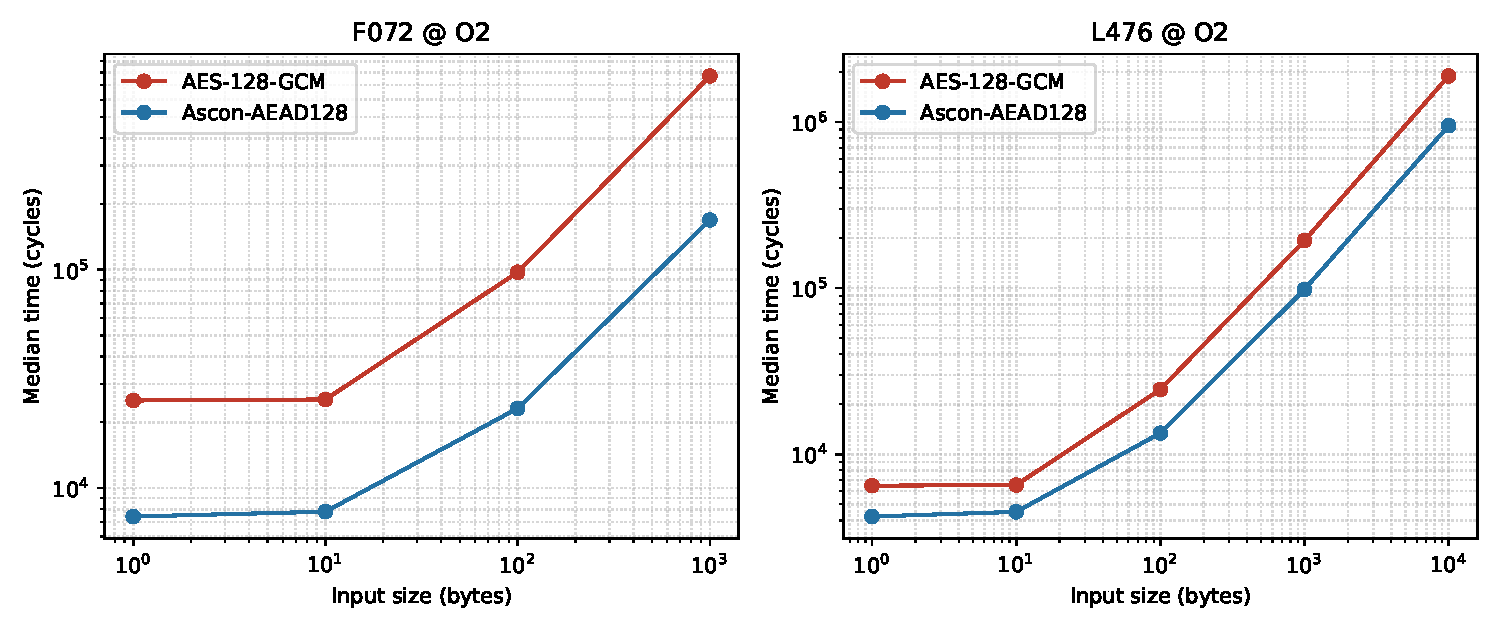
\includegraphics[width=\linewidth]{runtime_vs_size_O2}
  \caption{Median execution time vs.\ message size at \texttt{-O2} on both
           boards (logarithmic axes). Ascon-AEAD128 is consistently faster than
           AES-128-GCM at every size.}
  \label{fig:runtime}
\end{figure}

\subsection{Effect of Optimization Level}

Figure~\ref{fig:optsweep} shows median execution time at a fixed message size of
1000 bytes across the five optimization levels, with one panel per board and a
logarithmic time axis.
Table~\ref{tbl:timing-1000} gives the underlying values.

\begin{figure}[htbp]
  \centering
  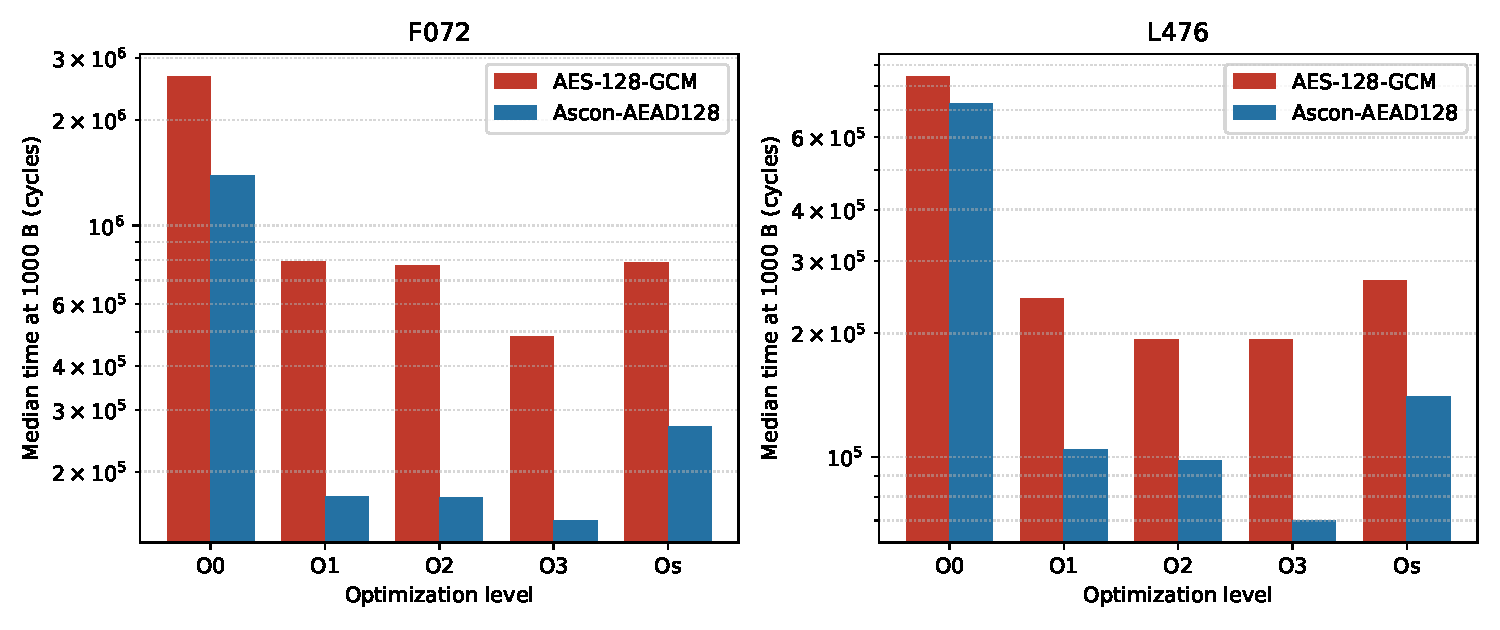
\includegraphics[width=\linewidth]{opt_sweep_1000B}
  \caption{Median execution time at 1000\,bytes across optimization levels on
           both boards (logarithmic time axis).}
  \label{fig:optsweep}
\end{figure}

The dominant effect is the step from \texttt{-O0} to \texttt{-O1}.
On the Cortex-M0 the Ascon-AEAD128 time at 1000 bytes falls from 1{,}387{,}063
cycles at \texttt{-O0} to 170{,}741 cycles at \texttt{-O1}, a factor of about
eight.
The AES-128-GCM time falls from 2{,}661{,}457 to 792{,}911 cycles over the same
step, a factor of about three.
On the Cortex-M4F the same step takes Ascon-AEAD128 from 726{,}789 to 104{,}422
cycles and AES-128-GCM from 845{,}537 to 242{,}980 cycles.

Between \texttt{-O1}, \texttt{-O2}, and \texttt{-O3} the changes are smaller
and not uniform.
On the Cortex-M4F, AES-128-GCM is essentially unchanged from \texttt{-O2} to
\texttt{-O3} (193{,}311 and 193{,}283 cycles), while Ascon-AEAD128 improves
from 98{,}262 to 70{,}194 cycles.
On the Cortex-M0, AES-128-GCM improves notably at \texttt{-O3}, from 770{,}536
to 485{,}227 cycles, while Ascon-AEAD128 improves modestly, from 168{,}921 to
145{,}888 cycles.

At \texttt{-Os} both algorithms are slower than at \texttt{-O2} on both boards.
On the Cortex-M0 the Ascon-AEAD128 time at \texttt{-Os} is 268{,}899 cycles,
slower than its \texttt{-O1} time.
On the Cortex-M4F the corresponding \texttt{-Os} time is 139{,}993 cycles.

\begin{table}[htbp]
  \centering
  \caption{Median execution time (cycles) and ratio at 1000\,bytes per
           optimization level.}
  \label{tbl:timing-1000}
  \begin{tabular}{lrrrrrr}
    \toprule
    Level &
    \multicolumn{1}{c}{M0 ASCON} &
    \multicolumn{1}{c}{M0 AES} &
    \multicolumn{1}{c}{M0 ratio} &
    \multicolumn{1}{c}{M4 ASCON} &
    \multicolumn{1}{c}{M4 AES} &
    \multicolumn{1}{c}{M4 ratio} \\
    \midrule
    \texttt{-O0} & 1{,}387{,}063 & 2{,}661{,}457 & 1.92 & 726{,}789 & 845{,}537 & 1.16 \\
    \texttt{-O1} &   170{,}741   &   792{,}911   & 4.64 & 104{,}422 & 242{,}980 & 2.33 \\
    \texttt{-O2} &   168{,}921   &   770{,}536   & 4.56 &  98{,}262 & 193{,}311 & 1.97 \\
    \texttt{-O3} &   145{,}888   &   485{,}227   & 3.33 &  70{,}194 & 193{,}283 & 2.75 \\
    \texttt{-Os} &   268{,}899   &   787{,}284   & 2.93 & 139{,}993 & 269{,}250 & 1.92 \\
    \bottomrule
  \end{tabular}
\end{table}

At \texttt{-O0} the two algorithms are close, especially on the Cortex-M4F
where the ratio is 1.16.
Once optimization is enabled the ratio is larger, and at every optimized level
the ratio is greater on the Cortex-M0 than on the Cortex-M4F.
The largest ratio in favor of Ascon-AEAD128 occurs at \texttt{-O1} and
\texttt{-O2} on the Cortex-M0, at approximately 4.6.

\section{Throughput}
\label{sec:throughput}

Figure~\ref{fig:cpb} shows median cycles per byte against input size on
logarithmic axes, with one panel per board, at \texttt{-O2}.
At the smallest size the cost per byte is highest, because the fixed per-call
cost is divided across a single byte.
As the message grows the cost per byte falls toward a flat asymptote, which is
the per-byte encryption rate.

\begin{figure}[htbp]
  \centering
  
\includegraphics[width=\linewidth]{cycles_per_byte_O2}
  \caption{Median cycles per byte vs.\ message size at \texttt{-O2} on both
           boards (logarithmic axes). The asymptotic value at large sizes
           reflects the steady-state per-byte encryption rate.}
  \label{fig:cpb}
\end{figure}

In the large-message region the per-byte rates at \texttt{-O2} are as follows.
On the Cortex-M0 at 1000 bytes, Ascon-AEAD128 reaches approximately 169 cycles
per byte and AES-128-GCM approximately 771 cycles per byte.
On the Cortex-M4F at 10{,}000 bytes, Ascon-AEAD128 reaches approximately
95 cycles per byte and AES-128-GCM approximately 189 cycles per byte.

At the smallest message size of one byte, where the figure reflects the fixed
per-call cost, the values at \texttt{-O2} are 7{,}410 cycles for Ascon-AEAD128
and 25{,}185 cycles for AES-128-GCM on the Cortex-M0, and 4{,}219 cycles for
Ascon-AEAD128 and 6{,}470 cycles for AES-128-GCM on the Cortex-M4F.

\section{Code Size}
\label{sec:code-size}

Figure~\ref{fig:footprint} shows the marginal Flash cost of each algorithm at
\texttt{-Os} for both boards.
Table~\ref{tbl:footprint} gives the marginal Flash cost at every optimization
level.

\begin{figure}[htbp]
  \centering
  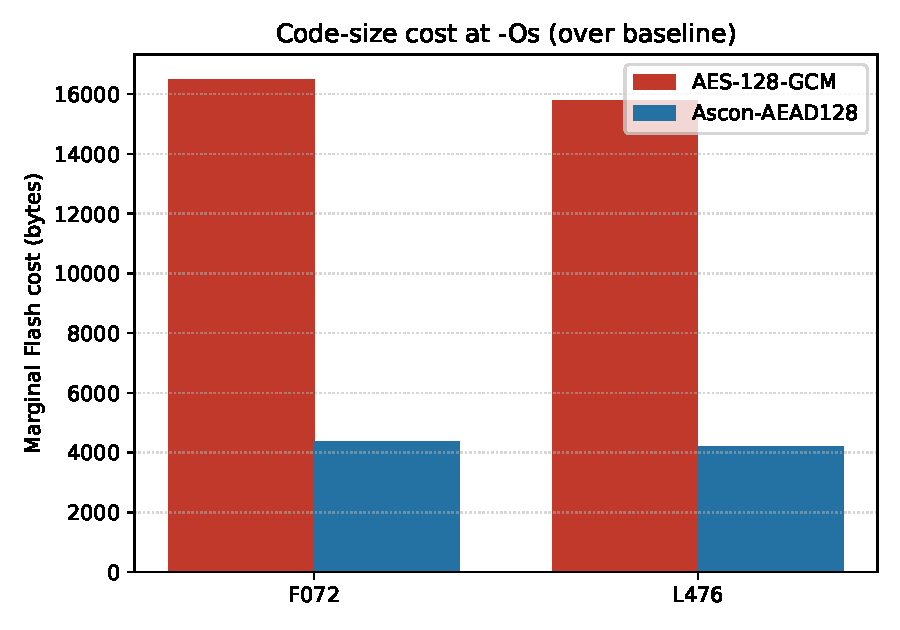
\includegraphics[width=0.75\linewidth]{footprint_flash_Os}
  \caption{Marginal Flash cost at \texttt{-Os} for each algorithm and board.
           Ascon-AEAD128 requires approximately 3.8$\times$ less Flash than
           AES-128-GCM at this level.}
  \label{fig:footprint}
\end{figure}

At \texttt{-Os}, Ascon-AEAD128 adds 4{,}376 bytes of Flash on the Cortex-M0
and 4{,}208 bytes on the Cortex-M4F.
AES-128-GCM adds 16{,}500 bytes on the Cortex-M0 and 15{,}776 bytes on the
Cortex-M4F.
The ratio of AES-128-GCM to Ascon-AEAD128 marginal Flash is approximately 3.8
on both boards.

\begin{table}[htbp]
  \centering
  \caption{Marginal Flash cost (bytes) and ratio per optimization level.}
  \label{tbl:footprint}
  \begin{tabular}{lrrrrrr}
    \toprule
    Level &
    \multicolumn{1}{c}{M0 AES} &
    \multicolumn{1}{c}{M0 ASCON} &
    \multicolumn{1}{c}{M0 ratio} &
    \multicolumn{1}{c}{M4 AES} &
    \multicolumn{1}{c}{M4 ASCON} &
    \multicolumn{1}{c}{M4 ratio} \\
    \midrule
    \texttt{-O0} & 26{,}296 & 12{,}836 & 2.05 & 23{,}256 &  6{,}776 & 3.43 \\
    \texttt{-O1} & 17{,}396 & 27{,}924 & 0.62 & 16{,}496 & 24{,}208 & 0.68 \\
    \texttt{-O2} & 17{,}476 & 27{,}504 & 0.64 & 16{,}584 & 23{,}264 & 0.71 \\
    \texttt{-O3} & 24{,}208 & 43{,}024 & 0.56 & 17{,}720 & 34{,}560 & 0.51 \\
    \texttt{-Os} & 16{,}500 &  4{,}376 & 3.77 & 15{,}776 &  4{,}208 & 3.75 \\
    \bottomrule
  \end{tabular}
\end{table}

The Ascon-AEAD128 marginal Flash cost varies strongly with optimization level.
Figure~\ref{fig:footprint-levels} shows this for each board.
At \texttt{-Os} it is the smaller of the two algorithms by a wide margin.
At \texttt{-O1}, \texttt{-O2}, and \texttt{-O3} it is larger than the
AES-128-GCM cost, reaching a maximum at \texttt{-O3} of 43{,}024 bytes on the
Cortex-M0 and 34{,}560 bytes on the Cortex-M4F.
The AES-128-GCM marginal Flash cost is comparatively stable across levels,
between roughly 16{,}000 and 26{,}000 bytes.
The shape of the Ascon-AEAD128 curve is the same on both boards, rising from
\texttt{-O0} through a peak at \texttt{-O3} and then falling sharply at
\texttt{-Os}.

\begin{figure}[htbp]
  \centering
  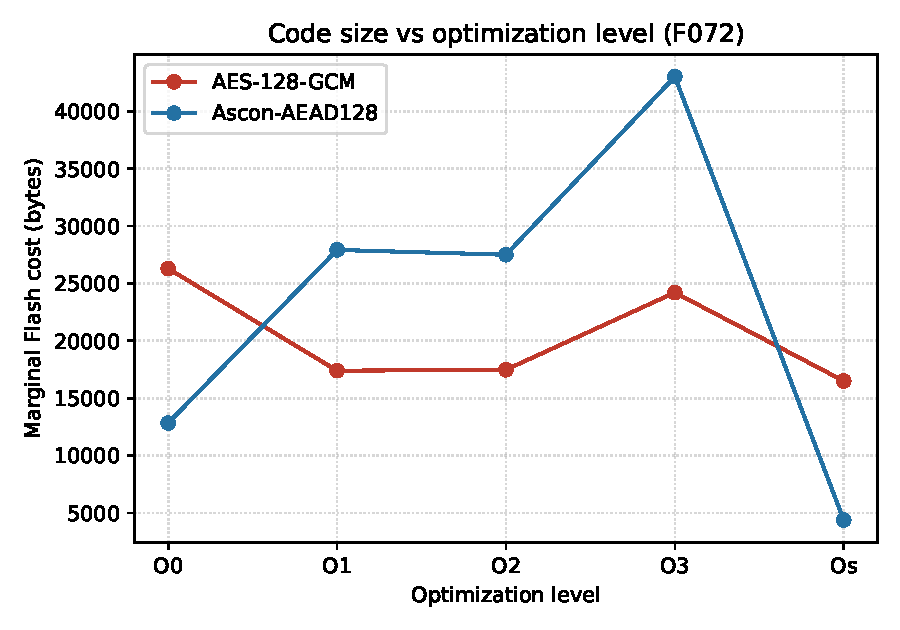
\includegraphics[width=0.49\linewidth]{footprint_across_levels_F072}%
  \hfill%
  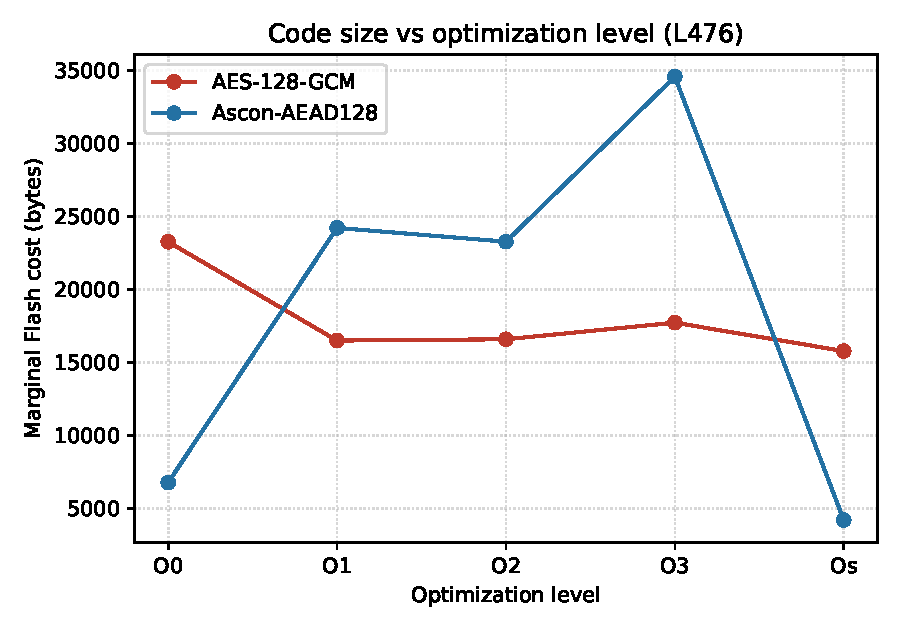
\includegraphics[width=0.49\linewidth]{footprint_across_levels_L476}
  \caption{Marginal Flash cost across all optimization levels. Left:
           Cortex-M0 (F072). Right: Cortex-M4F (L476). The Ascon-AEAD128
           cost varies strongly with optimization level due to permutation
           unrolling, while AES-128-GCM remains comparatively stable.}
  \label{fig:footprint-levels}
\end{figure}

\section{Summary of Results}

Across both boards and all message sizes, Ascon-AEAD128 executed faster than
AES-128-GCM at every optimization level.
The advantage was smallest at \texttt{-O0} and larger once optimization was
enabled.
At equal clock frequency the advantage was consistently larger on the Cortex-M0
than on the Cortex-M4F, reaching a factor of about 4.6 at 1000 bytes on the
Cortex-M0.
In code size, Ascon-AEAD128 was substantially smaller than AES-128-GCM at
\texttt{-Os}, by a factor of about 3.8 on both boards, while at the
speed-oriented optimization levels its reference implementation was larger than
AES-128-GCM due to the expansion of the permutation code.
These results are interpreted in relation to the four research questions in
Chapter~5.

\chapter{Discussion}

\section{Performance (Research Question 1)}

The first research question asks how the two algorithms compare in execution
time and throughput across message sizes on each platform.
The measurements give a clear answer: Ascon-AEAD128 was faster than AES-128-GCM
at every measured message size, on both boards, and at every optimization level.
The advantage was present in both the fixed per-call cost that dominates short
messages (Section~\ref{sec:exec-time}) and the per-byte cost that dominates long
messages (Section~\ref{sec:throughput}).
Ascon-AEAD128 leads in both regimes, so the conclusion does not depend on the
message-size profile of the application.

The reason for the difference lies in the structure of the two algorithms.
AES in software relies on table lookups for the substitution step, and the GCM
authentication step performs a multiplication in a binary field, built from many
smaller operations when no wide hardware multiplier is available.
Ascon-AEAD128 is built from a permutation of bitwise operations, exclusive-or,
bitwise-and, and rotation, applied to a small state held in registers.
These operations are native to both cores and require no table memory.
The single-pass duplex construction also avoids the separate encryption and
authentication passes that AES-128-GCM performs.
The measured advantage is the practical consequence of this design difference.

\section{Flash Footprint (Research Question 2)}

The second research question asks about the Flash footprint of each
implementation relative to the constraints of a small microcontroller.
The answer depends on the optimization level, and the size-optimized level is
the one relevant to a memory-constrained deployment.
At \texttt{-Os}, AES-128-GCM required approximately 3.8 times the code space of
Ascon-AEAD128, consistently on both boards (Section~\ref{sec:code-size}).
The small code size of Ascon-AEAD128 follows from its single permutation and its
lack of precomputed lookup tables, whereas AES-128-GCM brings the AES tables
and the field-multiplication code.

This advantage at \texttt{-Os} does not hold at the speed-oriented optimization
levels, for the reason examined in Section~\ref{sec:optlevel}.
The footprint result is therefore reported at the optimization level that a
constrained deployment would actually choose, where Ascon-AEAD128 is both
smaller and, from the timing results, faster.

\section{Optimization Sensitivity (Research Question 3)}
\label{sec:optlevel}

The third research question asks how the compiler optimization level affects the
relative performance of the two algorithms.
The measurements show that the optimization level matters a great deal, in two
distinct ways.

The first concerns execution time.
The largest single improvement for both algorithms came from enabling
optimization at all --- the step from \texttt{-O0} to \texttt{-O1}.
At 1000 bytes on the Cortex-M0 this step reduced the Ascon-AEAD128 time by a
factor of about eight and the AES-128-GCM time by a factor of about three.
This uneven response means the relative advantage of Ascon-AEAD128 is
understated by any measurement taken at \texttt{-O0}.
A study that benchmarked only unoptimized code would have reported the two
algorithms as close --- with a ratio of 1.16 on the Cortex-M4F --- and would
have missed the larger advantage that appears under the optimization a real
build would use.
The choice to sweep the optimization level, rather than report a single level,
is justified by this observation.

The behavior at the higher levels was not uniform.
On the Cortex-M4F, AES-128-GCM gained nothing from \texttt{-O3} over
\texttt{-O2}, consistent with the common observation that aggressive
optimization yields little for table-driven code on these cores, while
Ascon-AEAD128 continued to improve at \texttt{-O3}.
On the Cortex-M0 the pattern was reversed, with AES-128-GCM improving
substantially at \texttt{-O3} and Ascon-AEAD128 improving only modestly.
The \texttt{-Os} level was slower than \texttt{-O2} for both algorithms on both
boards, because size optimization disables the inlining and loop unrolling that
the cryptographic inner loops benefit from.

The second way the optimization level matters concerns code size, and it is the
more striking effect.
The Flash cost of the Ascon-AEAD128 reference implementation varied strongly
with the optimization level, while the AES-128-GCM cost was comparatively
stable.
The Ascon-AEAD128 cost rose from \texttt{-O0} to a peak at \texttt{-O3},
reaching 43{,}024 bytes on the Cortex-M0 and 34{,}560 bytes on the Cortex-M4F,
then fell sharply at \texttt{-Os} to roughly 4\,KB.
The cause is the unrolling of the permutation: at the speed-oriented levels the
compiler unrolls the permutation rounds into straight-line code, which the
authenticated-encryption routine includes at several call sites, expanding the
binary.
At \texttt{-Os} the compiler keeps the rounds rolled, and the code collapses to
a small size.
The same shape appeared on both boards, showing that the effect is a property
of the implementation and the compiler rather than of the processor.

This links the second and third research questions.
The footprint advantage of Ascon-AEAD128 is real but conditional on the
optimization level: it exists at \texttt{-Os} and is reversed at the
speed-oriented levels.
The advantage and this condition should be reported together.

\section{Architecture Dependence (Research Question 4)}

The fourth research question asks whether the performance gap between the two
algorithms differs between the Cortex-M0 and the Cortex-M4F, and what this
implies for device selection.
The measurements show that the gap is consistently larger on the weaker core.

At equal clock frequency and at 1000 bytes, the ratio of AES-128-GCM time to
Ascon-AEAD128 time was about 4.6 at \texttt{-O1} and \texttt{-O2} on the
Cortex-M0, against about 2.0 at the same levels on the Cortex-M4F.
At every optimized level the ratio was larger on the Cortex-M0.
The advantage of Ascon-AEAD128 therefore grows as the processor becomes more
constrained.

This can be read against the architectural baseline established in the harness
validation.
For the plain memory workload the Cortex-M0 was about 2.8 times slower than
the Cortex-M4F at the same clock.
If both algorithms simply scaled with this architectural factor, their ratio to
each other would be the same on both boards.
The fact that the AES-128-GCM disadvantage grows by more than this factor on
the Cortex-M0 indicates that AES-128-GCM contains operations that are
especially costly on the weaker core.
The field multiplication in the GCM authentication step is the principal
example: it must be synthesized from many small operations when no wide
hardware multiplier is present, which is the case on the Cortex-M0.
Ascon-AEAD128, built from operations the Cortex-M0 executes natively, stays
closer to the architectural baseline.

The implication for device selection is direct: the more constrained the
processor, the stronger the case for Ascon-AEAD128 over AES-128-GCM.
On the lowest-end cores, which are also the most numerous and the most
cost-sensitive, the advantage is largest.

\section{The Fairness of the Comparison}

The comparison was designed to avoid handicapping either algorithm, and one
configuration choice deserves explicit defense.
AES-128-GCM was measured with the small field-multiplication table, the
memory-frugal configuration disclosed in Section~3.4.1.
The larger table would improve throughput at a RAM cost that Ascon-AEAD128 does
not require, and on a part with 16\,KB of SRAM that is exactly the kind of cost
a constrained deployment may decline.

The reported AES-128-GCM figures therefore represent the memory-frugal end of
AES-128-GCM rather than its fastest possible configuration.
Enabling the larger table would narrow the throughput gap at large messages, at
a RAM cost Ascon-AEAD128 does not pay, and would not change the code-size or
small-message conclusions.
The comparison is thus a fair one between two lightweight configurations, and
the configuration choice is named and justified so the result cannot be read as
a weakened AES-128-GCM.

\section{Practical Conclusions}

The results support a consistent practical recommendation for the class of
devices studied.
For authenticated encryption on a constrained microcontroller without hardware
AES acceleration, Ascon-AEAD128 is the stronger choice on the measured criteria:
it was faster than AES-128-GCM at every message size and optimization level,
smaller in code at the size-optimized level that such a device would use, and
its advantage was largest on the most constrained processor.

Two qualifications accompany this recommendation.
First, the speed advantage and the size advantage do not occur at the same
optimization level for the reference implementation.
The size advantage holds at \texttt{-Os}, where Ascon-AEAD128 is both smaller
and faster than AES-128-GCM, so a deployment that builds for size obtains both
benefits at once.
A deployment that builds for speed at \texttt{-O2} or \texttt{-O3} obtains the
speed advantage but accepts a larger Ascon-AEAD128 code size due to the
unrolling of the permutation.
Second, these conclusions concern software-only implementations.
On a device with a hardware AES accelerator the balance would differ, and that
case was deliberately outside the scope of this work in order to isolate the
software comparison.

Within those qualifications, the measurements give a quantitative basis for
preferring Ascon-AEAD128 on constrained, software-only targets, and they
quantify how the advantage grows as the device becomes more limited.

\chapter{Conclusion and Outlook}

\section{Conclusion}

This work presented a measurement-based comparison of Ascon-AEAD128 and
AES-128-GCM on a Cortex-M0 and a Cortex-M4F, using software-only implementations
under matched conditions.
It was motivated by the absence of quantitative performance data for the
standardized lightweight algorithm on representative constrained hardware, and it
set out to provide that data across execution time, code size, optimization
level, and processor architecture.

The measurements answer the four research questions consistently: Ascon-AEAD128
was faster at every message size and optimization level on both boards, required
about one quarter of the Flash of AES-128-GCM at the size-optimized level, showed
an advantage that was understated at \texttt{-O0} and clearer once optimization
was enabled, and showed an advantage that grew on the more constrained
Cortex-M0.
Taken together the results give a quantitative basis for preferring
Ascon-AEAD128 on constrained, software-only targets, subject to the
qualification that the speed advantage and the code-size advantage are obtained
together only when building for size.

\section{Outlook}

Several directions extend this work.
First, measuring the larger-table AES-128-GCM configuration would bound the
fastest AES-128-GCM throughput achievable on these boards and quantify the speed
gained for the additional RAM.
Second, running the Cortex-M4F at its native 80\,MHz would give wall-clock
figures for that board at full speed, confirming the cycle-count results that
are independent of operating frequency.
Third, comparing Ascon-Hash256 against SHA-256 on the same hardware would extend
the comparison to the hashing use case that arises in key derivation and
integrity checking.
Fourth, repeating the study on a part with a hardware AES accelerator would
characterize how that shifts the balance and would mark the boundary of the
recommendation made here.
Fifth, measuring Ascon-80pq, which shares the same permutation as
Ascon-AEAD128~\cite{ASCONSpec}, would quantify the cost of its longer key and
position the comparison against longer-term security requirements.
These directions all build on the measurement infrastructure established here,
which was validated, frozen, and documented for reproducibility.


\bibliographystyle{IEEEtran}
\bibliography{references}
\end{document}
